\documentclass[a4paper,12pt]{article} % Changer la taille de police c'est ici

\usepackage{framed} % Marges
\usepackage[utf8]{inputenc} %francais
\usepackage[T1]{fontenc} %francais
\usepackage[french]{babel}  %francais
\usepackage{lmodern} % Pour changer le pack de police
\usepackage{makeidx} % Index
\usepackage{graphicx} % Figures
\usepackage{wrapfig} % Figures
\usepackage{amsmath} % Maths
\usepackage{amssymb} % symboles ?
\usepackage{bclogo} % ?????
\usepackage{stmaryrd}
\usepackage[top=2cm, bottom=2cm, left=2cm, right=2cm]{geometry} %Marges

\title{Rapport Tache 5 a}
\author{Interpolaspline}
\date{Avril 2020}

\begin{document}

\maketitle

\section{Introduction}

\section{Objectif}

Dans cette partie, il est question de la suppression des points aberrants avant le procédé d'interpolation.

Ici, la définition des points aberrants n'est pas fixe, les algorithmes développés en sont indépendants.

\section{Implémentation}

\subsection{algorithmes}

Le premier algorithme créé prend en argument une liste d'ordonnées et une méthode de détection des points aberrants, et traite toute la liste.

Dans un second temps, un deuxième algorithme a été créé, permettant de ne traiter que le point d'indice i. Cela permettra à l'avenir de reprendre cet algorithme pour supprimer les points aberrants pendant l'interpolation.

\subsection{tests}

Les tests ont été réalisés sur la définition des points aberrant suivante :

\emph{Un point est dit aberrant lorsqu'il n'appartient pas à l'intervalle }
\[[Q_1 - 1.5*(Q_3 - Q_1) , Q_3 +1.5*(Q_3 - Q_1)]\]

Le résultat est visible dans la figure \ref{suppr}.


\begin{figure}
\begin{center}
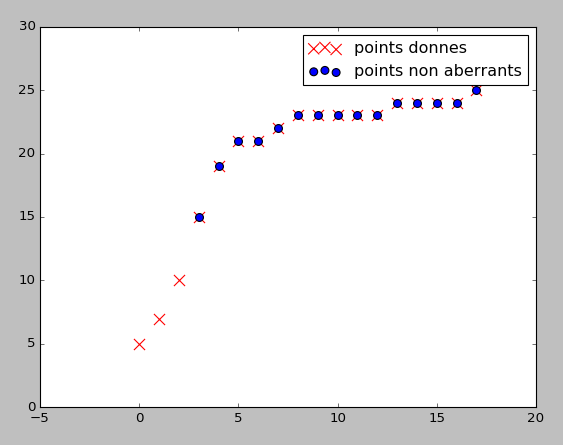
\includegraphics[width=8cm]{tache5a.png} 
\end{center}
\caption{Exemple de traitements des données}
\label{suppr}
\end{figure}

\end{document}
